% !TeX root = METOD.tex
\chapter{Идеальный газ.}

\emph{Идеальным газом} называется простейшая модель реального газа, в
которой делаются следующие допущения:

\begin{enumerate}
\def\labelenumi{\arabic{enumi}.}
\item
  Молекулы не имеют размеров, т. е. представляют собой материальные
  точки.
  \item
  Молекулы взаимодействуют друг с другом только путем упругих
  соударений.
\item
  Взаимодействие молекул на расстоянии отсутствует.
\end{enumerate}

\emph{Экспериментально} для постоянной массы идеального газа установлены
следующие законы:

\begin{enumerate}
\def\labelenumi{\arabic{enumi}.}
\item \emph{Закон Бойля-Мариотта} : при $T = const\quad pV = const.$
\item \emph{Закон Гей-Люссака} : при $P = const\quad V/T = const.$
\item \emph{Закон Шарля :} при $V = const\quad p/T = const.$
\end{enumerate}

Клапейроном был установлен объединенный газовый закон \emph{(уравнение
Клапейрона):}

\emph{Для постоянной массы газа} \[\frac{PV}{T} = const\]

Вид константы в этом уравнении был получен Менделеевым. Уравнение
состояния идеального газа \emph{(уравнение Менделеева-Клапейрона)} имеет
вид: 
\begin{equation}
  PV = \frac{m}{M}RT
\end{equation}

Здесь $R$~---~универсальная газовая постоянная ($R$ = 8,31 Дж /
(моль$\cdot$К)), $M$~---~молярная масса газа.

\emph{Моль} - количество вещества, в котором содержится столько молекул,
сколько их содержится в 12 г изотопа углерода С\textsuperscript{12}.%TODO: требуется уточнение этого понятия
Соответственно \emph{молярная масса} вещества равна его относительной
молекулярной массе, выраженной в граммах. Моль любого вещества содержит
\emph{число Авогадро} молекул
\begin{center}
  (\emph{N\textsubscript{A}} = 6,02 $\cdot$ 10\textsuperscript{23} моль\textsuperscript{-1}).
\end{center}

Для адиабатического процесса в идеальном газе справедливо \emph{уравнение Пуассона:}

$$PV^\gamma = const,$$
где \emph{γ = С\textsubscript{p}
/C\textsubscript{v}} - показатель адиабаты.

Для смеси газов справедлив \emph{закон Дальтона} :

Давление $P$, оказываемое смесью газов на стенки сосуда, равно сумме парциальных давлений всех компонент смеси, т.е. $P=\sum P_i$, где $P_i$~---~\emph{парциальное давление}
$i$-ой компоненты смеси, т.е. давление, которое оказывал бы на
стенки сосуда имеющийся в смеси газ, если бы он один занимал весь сосуд.
\begin{center}
  \textbf{Контрольные вопросы:}
\end{center}

\begin{enumerate}
\def\labelenumi{\arabic{enumi}.}
\item При каких условиях для смеси газов выполняется закон Дальтона?
\item Выведите закон Архимеда, используя формулу Торричелли и закон Паскаля.
\item Обоснуйте, почему единица количества вещества 1 моль выбрана именно
  таким способом.
\item Сформулируйте физический смысл универсальной газовой постоянной.
\item Объясните, что такое эффективная молярная масса смеси газов.
\item Укажите критерии применимости уравнения Менделеева-Клапейрона для
  описания реальных газов.
\end{enumerate}

\begin{center}
  \textbf{Литература}
\end{center}

{[}4{]} Гл. 1 . §4, §7.

{[}5{]} Гл. 1. §§ 2 - 4, §§ 7 - 9.

\begin{center}
  \textbf{Задачи}
\end{center}

\section{Найти эффективную молярную массу смеси двух идеальных
газов, для которых известны молярные массы \emph{М\textsubscript{1}} и
\emph{М\textsubscript{2}} и относительные массы \emph{a\textsubscript{1}
= m\textsubscript{1} / m} и \emph{a\textsubscript{2} =
m\textsubscript{2} / m,} где \emph{m = m\textsubscript{1} +
m\textsubscript{2} -} масса смеси\emph{.}}

\solving{}

Смесь идеальных газов представляет собой идеальный газ, который
подчиняется уравнению Менделеева-Клапейрона
\begin{equation}
  PV = \frac{m}{M_\text{эфф.}}RT,
\end{equation}
в котором $M_\text{эфф.}$~---~это эффективная молярная масса
смеси.

Для каждого из газов запишем уравнение состояния
\begin{equation*} \label{stateEqForParts}
  P_1V = \frac{m_1}{M_1}RT, \quad P_2V = \frac{m_2}{M_2}RT,
\end{equation*}
Складывая почленно уравнения \ref{stateEqForParts}, находим
\begin{equation*}
  (P_1+P_2)V = \left (\frac{m_1}{M_1}+\frac{m_2}{M_2} \right )RT.
\end{equation*}
По закону Дальтона для смеси газов $P = P_1 +P_2$.

Таким образом получаем: 
\begin{equation*}
  \frac{m}{M_\text{эфф.}} = \frac{m_1}{M_1} + \frac{m_2}{M_2}.
\end{equation*}
Отсюда 
\begin{equation}
  M_\text{эфф.} = \frac{m}{m_1/M_1 + m_2/M_2} = \frac{1}{a_1/M_1 + a_2/M_2}.
\end{equation}

\section{На поверхности жидкости плотности $\rho$ плавает
цилиндрический тонкостенный стакан, наполовину погруженный в жидкость.
На сколько погрузится нижняя кромка стакана в жидкость, если его
поставить на поверхность жидкости вверх дном? Высота стакана $h$,
давление воздуха $\rho_0$. На какую глубину нужно
погрузить перевернутый стакан, чтобы он вместе с заключенным в нем воздухом пошел ко дну?}

\solving{}

Стакан находится в равновесии под действием двух сил~---~силы тяжести $mg$ и силы Архимеда $F_A$. $F_A = \rho_\text{ж}gV$, где $V$~---~объем
погруженной части стакана, равный $V = S h/2$. Следовательно, масса
стакана равна
\begin{equation}
  m = \rho_\text{ж} S h /2,
\end{equation}
где $S$~---~площадь поперечного сечения стакана.

Во втором случае, когда стакан перевернут вверх дном, объем вытесненной жидкости равен $S y$, где $y$~---~разность уровней воды и воздуха в стакане (см. рис. \ref{glassInWater}, б). Из условия равновесия стакана
следует, что в этом случае также $mg = F_A$. Масса
стакана неизменна, поэтому объем вытесненной жидкости в обоих случаях одинаков, а т.к. толщина стенок пренебрежимо мала, то $y = h/2$.

По закону Бойля-Мариотта для воздуха, заключенного в стакане, находим $P_0V_1 = PV_2$, где $V_1 = S h$~---~объем стакана, а $V_2 = S z$, где $z$~---~высота столба воздуха в перевернутом стакане.

Из рис. \ref{glassInWater}, б видно, что $z = h - \left ( x - \frac{h}{2} \right ) = \frac{3}{2} h - x$. Здесь $x$~---~глубина погружения нижней кромки стакана в жидкость.

Таким образом, давление воздуха в перевернутом стакане равно
\begin{equation}
  P = \frac{Sh}{\left (\frac{3}{2}h - x \right )S} P_0 = \frac{h}{\left (\frac{3}{2}h - x \right )} P_0.
\end{equation}
Это давление уравновешивается давлением воды на глубине $y = h /2$. Поэтому $p = p_0 + ρ g h/2$. Отсюда находим
глубину погружения нижней кромки стакана $x$:
\begin{equation}
  P_0 + \frac{\rho g h}{2} = \frac{h}{\left (\frac{3}{2}h - x \right )} P_0 \Rightarrow x = \frac{3h}{2} - \frac{2P_0h}{2P_0 + \rho g h}.
\end{equation}

\begin{figure}[htbp]
  \centering
  \begin{tikzpicture}
    %%%% Первый случай
    \fill[cyan!10] (0,0) -- (0,2) -- (0.5,2) -- (0.5,1) -- (3.5,1) -- (3.5,2) -- (4,2) -- (4,0);
    \draw[thick] (0.5,3) -- (0.5,1) -- (3.5,1) -- (3.5,3);
    \draw (3.5,2) -- (4,2);
    \draw (3.5,1) -- (4,1);
    \draw[<->] (3.75,1) -- (3.75,2) node[pos=.5, xshift=5pt] {$\frac{h}{2}$};
    \node at (0.25,2.5) {а)};
    %%%% Второй случай
    \setcounter{shift}{5}
    \fill[cyan!10] (0+\theshift,0) -- (0+\theshift,2) -- (0.5+\theshift,2) -- (0.5+\theshift,1) -- (3.5+\theshift,1) -- (3.5+\theshift,2) -- (4.5+\theshift,2) -- (4.5+\theshift,0);
    \draw[thick] (0.5+\theshift,.25) -- (0.5+\theshift,2.25) -- (3.5+\theshift,2.25) -- (3.5+\theshift,.25);
    \draw (3.5+\theshift,2) -- (4.5+\theshift,2);
    \draw (3.5+\theshift,1) -- (4+\theshift,1);
    \draw (3.5+\theshift,.25) -- (4.5+\theshift,.25);
    \draw[<->] (3.75+\theshift,1) -- (3.75+\theshift,2) node[pos=.5, xshift=5pt] {$y$};
    \draw[<->] (4.25+\theshift,.25) -- (4.25+\theshift,2) node[pos=.5, xshift=5pt] {$x$};
    \node at (0.25+\theshift,2.5) {б)};
    %%%% Третий случай
    \setcounter{shift}{10.99}
    \fill[cyan!10] (0+\theshift,-1.5) -- (0+\theshift,2) -- (4+\theshift,2) -- (4+\theshift,-1.5);
    \fill[white] (0.5+\theshift,0) -- (0.5+\theshift,1) -- (3.5+\theshift,1) -- (3.5+\theshift,0);
    \draw[thick] (0.5+\theshift,-1) -- (0.5+\theshift,1) -- (3.5+\theshift,1) -- (3.5+\theshift,-1);
    \draw[<->] (2+\theshift,1) -- (2+\theshift,2) node[pos=.5, xshift=7pt] {$H$};
    \draw[<->] (2.5+\theshift,0) -- (2.5+\theshift,1) node[pos=.5, xshift=5pt] {$\frac{h}{2}$};
    \node at (0.25+\theshift,2.5) {в)};
  \end{tikzpicture}
  \caption{}
  \label{glassInWater}
\end{figure}

Для того, чтобы перевернутый стакан пошел на дно, надо погрузить его на такую глубину, на которой воздух в стакане будет сжат настолько, что его объем будет меньше минимального объема $V_{min.} = Sh/2$, определяемого из условия равновесия $mg = F_A$. При таком объеме воздуха в стакане сила тяжести будет больше архимедовой силы, и стакан будет тонуть. Давление воздуха в стакане равно давлению воды на глубине $H + h/2$ (см. рис. \ref{glassInWater}, в). Следовательно, получаем:

\begin{equation}
  P_0 + \rho g(H + h/2) = P = \frac{V_1}{V_{min}}P_0 = 2 P_0.
\end{equation}
Отсюда находим 
\begin{equation}
  P_0 = \rho g(H + h/2).
\end{equation}
Откуда 
\begin{equation}
  H = \frac{P_0}{\rho g} - \frac{h}{2}. 
\end{equation}

\section{В гладкой, открытой с обоих концов вертикальной трубе, имеющей два разных сечения (см. рис. \ref{thermometer}) находятся два поршня, соединенные нерастяжимой нитью, а между поршнями~---~один моль идеального газа. Площадь сечения верхнего поршня на \emph{∆ S} больше, чем нижнего.
Общая масса поршней \emph{m}. Давление наружного воздуха
\emph{p\textsubscript{0}}. На сколько нужно изменить температуру газа
между поршнями, чтобы они переместились на расстояние \emph{∆ z}.}

\solving{}

\begin{wrapfigure}[9]{R}{.4\textwidth}
  \centering
  \begin{tikzpicture}
    \draw[thick] (0,3) -- (0,1.5) -- (1,1.5) -- (1,0);
    \draw[thick] (5,3) -- (5,1.5) -- (4,1.5) -- (4,0);
    \draw[->] (5.5,0) -- (5.5,3) node [xshift=6pt] {$z$};
    \draw (5.4,1.5) -- (5.6,1.5) node [anchor=west] {$0$};
    \fill[yellow] (0,2.9) rectangle (5,2.75) node[pos=.7, anchor=north, black] {$S_2$};
    \filldraw[pattern=north east lines] (0,2.9) rectangle (5,2.75) node[pos=.5, anchor=south] {$P_0$};
    \fill[yellow] (1,.1) rectangle (4,.25) node[pos=.7, anchor=south, black] {$S_1$};
    \filldraw[pattern=north east lines] (1,.1) rectangle (4,.25) node[pos=.5,anchor=north] {$P_0$};
    \draw[ultra thick] (2.5,2.75) -- (2.5,.25) node[pos=.5,anchor=west] {$l$};
    \node at (1.7,1.7) {$P$};
  \end{tikzpicture}
  \caption{}
  \label{thermometer}
\end{wrapfigure}
Из условия механического равновесия системы <<поршни-нить>> следует: $P_0\Delta S + mg = P\Delta S$, где $P$~---~давление газа между поршнями.

Отсюда получаем:
\begin{equation} \label{PresMechEquilib}
  P = P_0 + \frac{mg}{\Delta S}.
\end{equation}
Отсюда можно сделать вывод, что процесс является изобарным, а значит:
\begin{equation} \label{StateEq}
  \Delta T = \frac{P}{R}\Delta V
\end{equation}
Объём внутри сосуда определятся как:
\begin{equation*} 
  V = zS_2 + (l - z)S_1 = lS_1 + z(S_2-S_1).
\end{equation*}
Видно, что $V$ от $z$ зависит линейно, а значит 
\begin{equation} \label{VolumeChange}
  \Delta V = \Delta z \Delta S
\end{equation}
Подставляя \ref{PresMechEquilib} и \ref{VolumeChange} в \ref{StateEq} получим 
\begin{equation}
  \Delta T = \left (P_0 + \frac{mg}{\Delta S}\right ) \frac{\Delta S}{R}\Delta z = \left (\frac{P_0 \Delta S + mg}{R}\right ) \Delta z
\end{equation}

Рассмотренное устройство может служить термометром с линейной шкалой в области $T > T_0$.

При $m = 5$ кг , $∆S = 10$ см\textsuperscript{2}, $\Delta z = 1$ см получаем $\Delta T \approx 0,2$ K.

Таким образом термометр оказывается весьма чувствительным.

\section{В вертикальном цилиндрическом сосуде находится в равновесии
тяжелый поршень. Над поршнем и под ним имеются одинаковые массы газа при
одинаковой температуре \emph{Т\textsubscript{0}} . Отношение верхнего
объема к нижнему равно \emph{n\textsubscript{0}} . При какой температуре
\emph{Т} отношение объемов станет равным \emph{n} ?}

\solving{}
\begin{wrapfigure}[7]{R}{.35\textwidth}
  \centering
  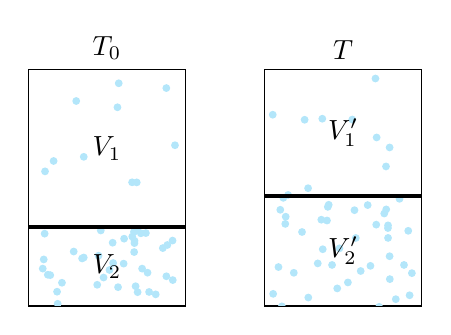
\begin{tikzpicture}
    % Первый случай
    \begin{scope}
      \draw[clip] (0,0) rectangle (2,3) ;
      \foreach \i in {1,2,...,10}{
        \node[circle,fill,inner sep=1pt,cyan!30] at (rand/1.1+1,rand/1.1+2) {};}
      \foreach \i in {1,2,...,40}{
        \node[circle,fill,inner sep=1pt,cyan!30] at (rand/1.1+1,rand/2.1+.5) {};}
      \draw[ultra thick] (0,1) -- (2,1); 
      \node at (1,2) {$V_1$};
      \node at (1,.5) {$V_2$};
    \end{scope}
    \node[anchor=south] at (1,3) {$T_0$};
    % Второй случай
    \begin{scope}
      \draw[clip] (3,0) rectangle (5,3);
      \foreach \i in {1,2,...,10}{
        \node[circle,fill,inner sep=1pt,cyan!30] at (rand/1.1+4,rand/1.1+2.1) {};}
      \foreach \i in {1,2,...,40}{
        \node[circle,fill,inner sep=1pt,cyan!30] at (rand/1.1+4,rand/1.4+.7) {};}
      \draw[ultra thick] (3,1.4) -- (5,1.4); 
      \node at (4,2.2) {$V_1'$};
      \node at (4,.7) {$V_2'$};
    \end{scope}
    \node[anchor=south] at (4,3) {$T$};
    \end{tikzpicture}
  \caption{}
  \label{<label>}
\end{wrapfigure}

Запишем уравнение Менделеева-Клапейрона для газа в первом и втором случаях:

В первом случае:
\begin{equation}
  \begin{aligned} \label{MendKlapEqFirst}
    P_1V_1 &= \frac{m}{M}RT_0, \\
    P_2V_2 &= \frac{m}{M}RT_0.
  \end{aligned}
\end{equation}
Во втором случае:
\begin{equation}
  \begin{aligned} \label{MendKlapEqSecond}
    P_1'V_1' &= \frac{m}{M}RT, \\
    P_2'V_2' &= \frac{m}{M}RT.
  \end{aligned}
\end{equation}

Из уравнений \ref{MendKlapEqFirst} следует, что 
\begin{equation} \label{nZero}
  \frac{P_2}{P_1} = \frac{V_1}{V_2} = n_0,
\end{equation}
а из уравнений \ref{MendKlapEqSecond} вытекает, что 
\begin{equation} \label{n}
  \frac{P_2'}{P_1'} = \frac{V_1'}{V_2'} = n.
\end{equation}

Разделив уравнения \ref{MendKlapEqFirst} на соответствующие уравнения \ref{MendKlapEqSecond}, получаем:
\begin{equation} \label{eq1}
  \frac{T}{T_0} = \frac{P_1'V_1'}{P_1V_1} = \frac{P_2'V_2'}{P_2V_2}.
\end{equation}

Отношение давлений газа над поршнем в первом и втором случаях находим,
используя условие механического равновесия поршня:
\begin{equation}
  P_2 = P_1 +\frac{mg}{S}, \quad P_2' = P_1' +\frac{mg}{S}
\end{equation}

Учитывая, что из уравнений \ref{nZero} и \ref{n} следуют соотношения:
\begin{equation}
  P_2 = n_0 P_1, \quad P_2' = n P_1',
\end{equation}
находим:
\begin{equation}
  P_2' - P_2 = P_1' - P_1 = nP_1' - n_0P_1.
\end{equation}
Отсюда получаем:
\begin{equation} \label{eq2}
  \frac{P_1'}{P_1} = \frac{n_0-1}{n-1}.
\end{equation}

Отношение объемов, занимаемых газом над поршнем в первом и втором
случаях, находим, учитывая, что полный объем сосуда в обоих случаях
одинаков:
\begin{equation} \label{VolumeSave}
  V_1 +V_2 = V_1' +V_2' \Rightarrow V_1 + \frac{V_1}{n_0} = V_1' + \frac{V_1'}{n}.
\end{equation}
Из выражения \ref{VolumeSave} получаем:
\begin{equation} \label{eq3}
  \frac{V_1'}{V_1} = \frac{n(n_0+1)}{n_0(n+1)}.
\end{equation}
Из выражений \ref{eq1}, \ref{eq2} и \ref{eq3} находим:
\begin{equation} \
  T = T_0\frac{n(n_0^2-1)}{n_0(n^2-1)}.
\end{equation}

\section{Горизонтально расположенный цилиндрический сосуд сечением
\emph{S} и длиной \emph{2l} содержит идеальный газ, давление которого
\emph{p\textsubscript{0}}, температура \emph{T\textsubscript{0}}.
Цилиндр разделен на две половины тонким поршнем массы \emph{m}, который
способен скользить вдоль цилиндра без трения. Найти период малых
колебаний поршня.}

\solving{}

\begin{figure}[htbp]
  \centering
  \begin{tikzpicture}
    \foreach \i in {1,2,...,30}{
        \node[circle,fill,inner sep=1pt,cyan!30] at (rand*2.53+2.54,rand*1.21+1.25) {};}
    \foreach \i in {1,2,...,30}{
        \node[circle,fill,inner sep=1pt,cyan!30] at (rand*1.8+7.1,rand*1.21+1.25) {};}
    \draw[->] (-.2,0) -- (10,0) node[anchor=north east] {$x$};
    \draw (0,0) rectangle (9,2.5);
    \draw[dashed] (4.5,2.5) -- (4.5,0) node[anchor=north] {$0$};
    \filldraw[pattern=north east lines] (5.1,0) rectangle (5.2,2.5);
    \draw[->] (5.1,1.25) -- (4.7,1.25) node [pos=0,anchor=south east] {$\vec{F}$};
    \node[anchor=north] at (0,0) {$-l$};
    \node[anchor=north] at (9,0) {$l$};
  \end{tikzpicture}
  \caption{}
  \label{pistonOscillation}
\end{figure}

Поршень будет совершать колебания, т.к. при выведении его из положения
равновесия равнодействующая сил давления газа $\vec{F}$ по обе стороны от поршня направлена
в сторону положения равновесия (рис. \ref{pistonOscillation}). В результате под действием
этой силы поршень стремится вернуться в исходное положение. В положении
равновесия эта сила обращается в нуль, но поршень по инерции проходит
это положение, т.к. его скорость в этот момент отлична от нуля.
Возникают колебания поршня.

Изменение давления газа при смещении поршня зависит от вида процесса.
Если процесс можно считать \emph{изотермическим}, то воспользовавшись
законом Бойля-Мариотта находим изменение давления газа при бесконечно
малом изменении объема сосуда на $dV$ :
\begin{equation}
  PV = const \Rightarrow d(PV) = 0 \Rightarrow dP= -P\frac{dV}{V}.
\end{equation}
Знак <<$-$>> означает, что увеличение объема приводит к уменьшению
давления в сосуде и наоборот.

В случае малых колебаний смещение поршня $x \ll l$. В этом случае для малых конечных изменений объема и давления имеем:
\begin{equation}
  \Delta P = - P_0\frac{\Delta V}{V} = -P_0\frac{x}{l}.
\end{equation}

Равнодействующая сил давления, действующих на поршень, равна:
\begin{equation}
  F = 2\Delta P\cdot S = -2SP_0\frac{x}{l}.
\end{equation}
Знак <<$-$>> указывает на то, что сила направлена в сторону
противоположную смещению поршня $x$.

Из второго закона Ньютона для поршня следует, что уравнение движение поршня имеет вид:
\begin{equation}
  a = \frac{d^2x}{dt^2} = \frac{F}{m} = -2SP_0\frac{x}{ml}.
\end{equation}

Отсюда приходим к уравнению
\begin{equation}
  \frac{d^2x}{dt^2}+\frac{2SP_0}{ml}x = 0.
\end{equation}

Тело, движение которого описывается таким уравнением, совершает
гармонические колебания с циклической частотой
\begin{equation}
  \omega = \sqrt{\frac{2SP_0}{ml}}.
\end{equation}
Отсюда период малых колебаний поршня равен:
\begin{equation}
  T = 2\pi\sqrt{\frac{ml}{2SP_0}}.
\end{equation}

Если колебания поршня происходят \emph{адиабатически}, то в этом случае изменение давления при смещении поршня определяем из уравнения Пуассона:
\begin{equation}
  PV^\gamma = const \Rightarrow d(PV^\gamma) = 0 \Rightarrow dP = - \gamma p \frac{dV}{V}.
\end{equation}
Соответственно сила, действующая на поршень, будет равна:
\begin{equation}
  F = 2 S \Delta P = - 2\gamma SP_0\frac{x}{l}.
\end{equation}
Уравнение движения примет вид:
\begin{equation}
  \frac{d^2x}{dt^2}+\frac{2\gamma SP_0}{ml}x = 0.
\end{equation} 
Период колебаний поршня в этом случае равен:
\begin{equation}
  T = 2\pi\sqrt{\frac{ml}{2\gamma SP_0}}.
\end{equation}

\section{\boldmath Поршневой воздушный насос емкости $\Delta V$ откачивает воздух из сосуда емкости $V$. За сколько циклов работы насоса давление понизится от $P_0$ до $P$. Процесс считать изотермическим.}

\section{Сделать приближенную оценку толщины земной атмосферы, приняв, что ее температура равна 300 К. \textup{\normalfont  Указание: сделать допущение, что плотность атмосферы постоянна.}}

\section{Герметически закрытый бак высоты 3 м полностью заполнен водой, только на дне его находятся два одинаковых пузырька воздуха. Давление на дно бака 0,15 МПа. Каким станет давление на дно, если всплывет один пузырек? Два пузырька?}

\section{\boldmath Нижний конец вертикальной узкой трубки длины $2l$ запаян, а верхний открыт в атмосферу. В нижней половине трубки находится газ при температуре $T_0$, а верхняя половина заполнена ртутью. До какой минимальной температуры надо нагреть газ в трубке, чтобы он вытеснил всю ртуть? Внешнее давление совпадает с давлением ртутного столба длины $l$.}

\section{\boldmath Коэффициент адиабатического расширения воздуха $\gamma$ можно измерить методом Клемана-Дезорма, при котором в сосуде, содержащем воздух, вначале увеличивают давление на небольшую величину $P_1 (P_1 \ll P_\text{атм.})$, а затем адиабатически понижают давление до атмосферного, кратковременно открыв сосуд. Через некоторое время после закрытия сосуда давление оставшегося в сосуде воздуха самопроизвольно понижается на величину $P_2 < P_1$. Коэффициент адиабаты вычисляется по формуле $\gamma = \frac{P_1}{P_1 - P_2}$. Доказать это соотношение.}